\documentclass[11pt]{article}

\usepackage[margin=1in]{geometry}
\usepackage{amsmath,amssymb,braket}
\usepackage{hyperref}
\usepackage{graphicx}

\begin{document}

\begin{center}
{\Large 5260--2026 Midterm Project: Numerical Experiments on Quantum Relaxation}\\[12pt]
Please submit \emph{typed} by 3/16/2026 (email pdf attachment to 
\texttt{anitzan@sas.upenn.edu} and \texttt{wying3@sas.upenn.edu})
\end{center}

\textbf{Note:} This is a research assignment. You can expand the scope of your research. For example, model A was shown, under certain assumptions, in class to lead to an exponential decay of the probability to stay in state 1 at time $t$. If you numerically get different results you can try to investigate why.

\bigskip
\hrule
\bigskip

\begin{figure}[htbp]
    \centering
    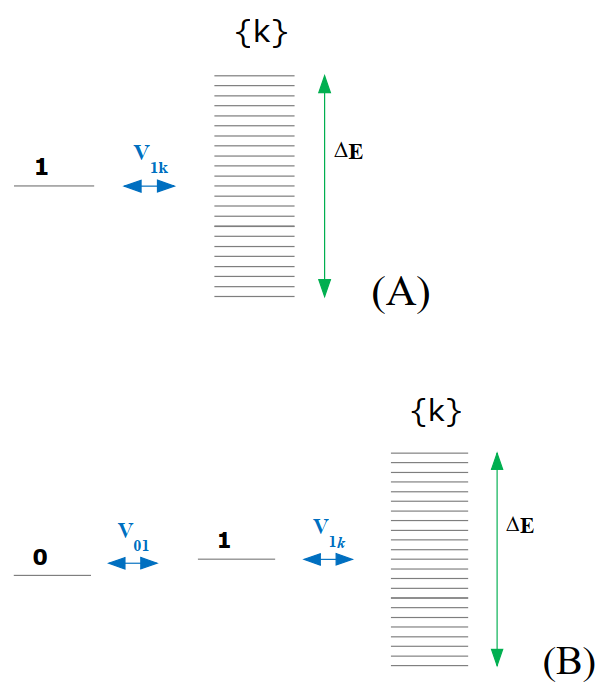
\includegraphics[width=0.45\linewidth]{Figure1.png}
    \caption{(A) (B)}
    \label{fig:1}
\end{figure}

~\\\\
Figures (A) and (B) show different models for which the time evolution of a quantum system needs to be investigated.
In each of these models the initial state of the system $|a\rangle$ is given and you need to calculate and plot as a function of time $t$ the probability $P_b(t) = |\braket{b|\Psi(t)}|^2$ that the system will be found in state $|b\rangle$ at time $t$. 

\subsection*{Model (A)}
The initial state is $\ket{1}$, and the Hamiltonian is 
\begin{equation*}
    \hat H = E_1\ket{1}\bra{1} + \sum_{k=0}^N E_k \ket{k}\bra{k} + \sum_{k=0}^N \left( V_{1k}\ket{1}\bra{k} + V_{k1}\ket{k}\bra{1} \right).
\end{equation*}
The total number of levels is $N+1$.

\subsection*{Model (B)}
The initial state is $\ket{0}$. The Hamiltonian is
\begin{align*}
    \hat H &= E_0\ket{0}\bra{0} + E_1\ket{1}\bra{1} + V_{01}\ket{0}\bra{1} + V_{10}\ket{1}\bra{0} + \sum_{k=0}^N E_k \ket{k}\bra{k} + \sum_{k=0}^N \left( V_{1k}\ket{1}\bra{k} + V_{k1}\ket{k}\bra{1} \right).
\end{align*}
The total number of levels is  $N+2$.

\bigskip\bigskip

\noindent Typical numbers to use are $N_K = 100$--$200$ but you can try to take more or less to examine the effects on your results.\\

\noindent Starting from $C_1(0)=1$ in model (A) and $C_0(0)=1$ in model (B), calculate and plot as functions of time:

\begin{itemize}
\item probability to remain in $\ket{1}$ at time $t$ for model (A).
\item probabilities to be in $\ket{0}$ and in $\ket{1}$ for model (B).
\item and also the overall probability $P_K(t)=\sum_k |\braket{k|\Psi(t)}|^2$ to be in the state $\ket{k}$. 
\end{itemize}
Investigate the behavior of your results for different choices of $\Delta E$ and the couplings $V$. 

\subsection*{Parameters to choose}
Take the span of the manifold $K$ to be $\Delta E$, between $E_1 \pm \Delta E/2$. The spacing between two nearest levels is $\epsilon = \Delta E / N \equiv \rho^{-1}$. Take all the coupling elements $V_{1k}$ to be (a) equal, and (b) equal in magnitude but random in sign. 
All the coupling parameters may be assumed real. If not, make sure you take $\{ V_{k1} = V_{1k}^* \}$, etc. Note that one of the energies, say $E_1$, may be taken 0 without loss of generality.\\

\noindent A typical coupling to use in Model (A) should be in the range $\Delta E \gg V_{1,k} \gg \rho^{-1}$ (explain why) but it would be nice to check what happens if you go beyond these limits.\\

\noindent You can take all $V_{1,k}$ to be the same (independent of $k$) but it will also be nice to investigate what happens when they come from a random distribution (for example assign random $\pm$ signs to the different matrix elements or, more generally, generate them from a random distribution so that $\langle V \rangle = 0$ and $\langle V^2 \rangle^{1/2}$ satisfies $\Delta E \gg \langle V^2 \rangle^{1/2} \gg \rho^{-1}$.\\

\noindent For each model compare these results for the two cases: The coupling matrix elements are (1) all equal or (2) equal in magnitude but with random sign. (More generally you generate them from a random distribution so that $\langle V \rangle = 0$ and $\langle V^2 \rangle^{1/2}$ satisfies $\Delta E \gg \langle V^2 \rangle^{1/2} \gg \rho^{-1}$). \\

\noindent Check the sensitivity of your results to the choice of $\Delta E$, $N$, $V_{1k}$, $V_{01}$, $E_0-E_1$ ($E_1$ may be taken 0 without loss of generality). \\

\noindent \underline{\bf Summarize your findings in a clear and systematic way.}

\end{document}
